\documentclass[12pt]{exam}
\usepackage{amsthm}
\usepackage{libertine}
\usepackage[utf8]{inputenc}
\usepackage[margin=1in]{geometry}
\usepackage{amsmath,amssymb}
\usepackage{multicol}
\usepackage[shortlabels]{enumitem}
\usepackage{siunitx}
\usepackage{cancel}
\usepackage{graphicx}
\usepackage{pgfplots}
\usepackage{listings}
\usepackage{tikz}


\pgfplotsset{width=10cm,compat=1.9}
\usepgfplotslibrary{external}
\tikzexternalize

\newcommand{\class}{Moderna - Complementaria} % This is the name of the course 
\newcommand{\examnum}{Tarea 3} % This is the name of the assignment
\newcommand{\examdate}{10/02/2023} % This is the due date
\newcommand{\timelimit}{}





\begin{document}
\pagestyle{plain}
\thispagestyle{empty}

\noindent
\begin{tabular*}{\textwidth}{l @{\extracolsep{\fill}} r @{\extracolsep{6pt}} l}
\textbf{\class} & \textbf{Name:} & \textit{David Pachon}\\ %Your name here instead, obviously 
\textbf{\examnum} && Sergio Montoya\\
\textbf{\examdate} &&\\
\end{tabular*}\\
\rule[2ex]{\textwidth}{2pt}
% ---




\begin{enumerate} %You can make lists!

	\item para esto vamos a partir de $u=\frac{u'+v}{1+\frac{u'v}{c^2}}$ y llegaremos al punto que nos interesa.
		\begin{align*}
			&u=\frac{u'+v}{1+\frac{u'v}{c^2}}\\
			&=(u'+v)(1+\frac{u'v}{c^2})^{-1}; \text{ Aqui utilizaremos la pista que se nos dio }\\
			&=(u'+v)(1-\frac{u'v}{c^2})\\
			&=u'-\frac{u'^{2}v}{c^2}+v-\frac{u'v^2}{c^2};\text{ Aqui vamos a utilizar que  } u' = \frac{c}{n}\\
			&=u'-\frac{\frac{c^{2}}{n}v}{c^2} + v - \frac{\frac{c}{n}v}{c^2}\\
			&=u'-\frac{v}{n^2}+v-\frac{v}{cn};\\
			&\text{ Este ultimo termino es 0 pues físicamente un fluido no puede ir a velocidades cercanas a la luz }\\
			&=u'+ v-\frac{v}{n^2}=u' + \left(1-\frac{1}{n^2}\right)v,\text{ QED }\\
		\end{align*}
	\item Lo primero que vamos a hacer es transformar las unidades que nos dieron a unas mas utiles.
		\begin{eqnarray*}
			x_{lab}=&9.5cm=&0.095 m\\
			t_{propio}=& 2.2\mu s=&2.2\times10^{-6}S
		\end{eqnarray*}
		Luego de esto, planteemos las ecuaciones con las que vamos a trabajar.
		\begin{eqnarray*}
			x_{lab}&=&V\cdot t_{lab}\\
			t_{lab}&=&\gamma \cdot t_{propio}
		\end{eqnarray*}
		Una vez tenemos esto vamos a desarrollar como sigue:
		\begin{align*}
			&x_{lab} = V \gamma t_{propio}\\
			&= v\frac{t_{propio}}{\sqrt{1-\frac{v^2}{c^2}}}\\
			&\frac{x_{lab}}{v}=\frac{t_{propio}}{\sqrt{1-\frac{v^2}{c^2}}}\\
			&\frac{v^2}{x_{lab}^2} = \frac{1-\frac{v^2}{c^2}}{t_{propio}}\\
			&v^2t_{propio}^2 = x^2_{lab}-\frac{x_{lab}^2v^2}{c^2}\\
			&v^2t_{propio}^2 +\frac{x_{lab}^2v^2}{c^2} = x_{lab}^2\\
			&v^{2}(t_{propio}^2+\frac{x_{lab}^2}{c^2}) = x_{lab}^2\\
			&v=\sqrt{\frac{x_{lab}}{t_{prop}^2+\frac{x_{lab}^2}{c^2}}}\\
			&v=\sqrt{\frac{(0.095)^2}{(2.2\times10^{-6})^2+\frac{0.095^2}{3\times10^{8}^2}}}\\
			&v=43181.8 \frac{m}{s}\\
			&v=\frac{43181.8}{3\times10^{8}}\\
			&v= 1.44\times10^{-4}C
		\end{align*}
	\item \begin{figure}
		\centering
		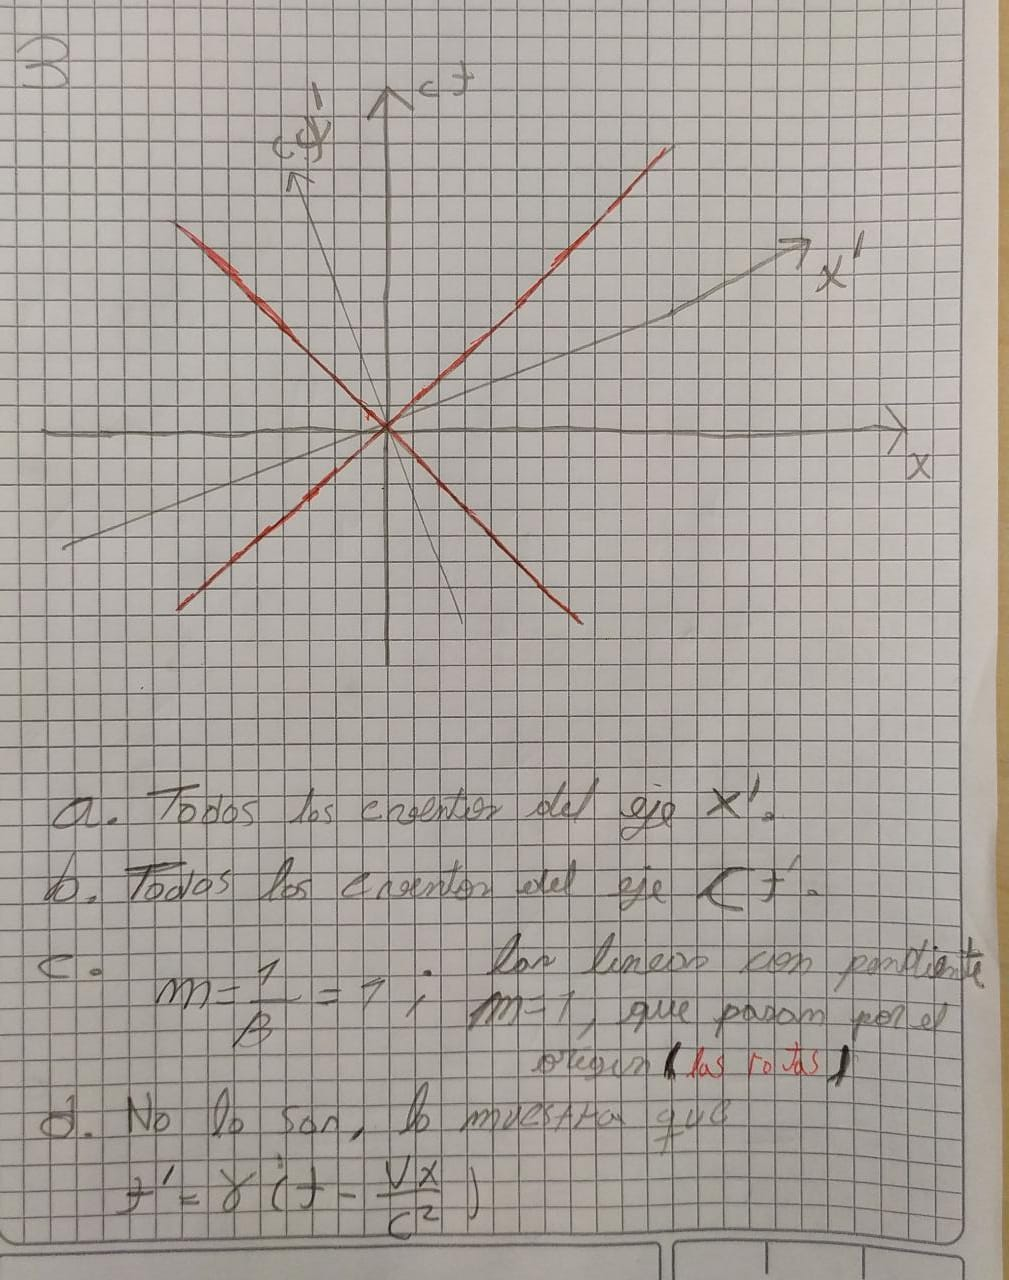
\includegraphics[scale=0.4]{Punto3.jpeg}
	\end{figure}
\end{enumerate}



\end{document}
